
\documentclass[12pt]{standalone}
\usepackage{tikz}
\usetikzlibrary{automata,positioning}
\begin{document}
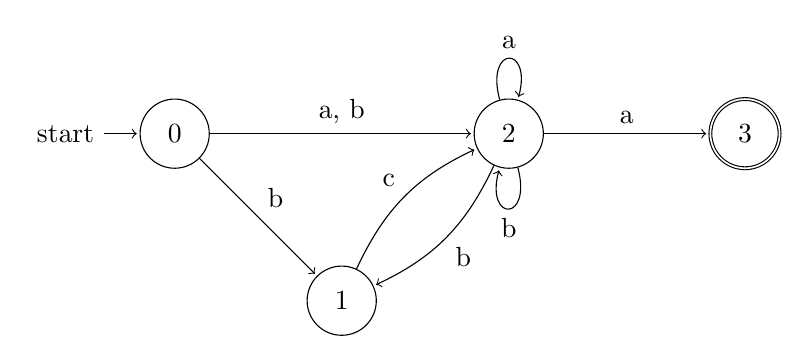
\begin{tikzpicture}[shorten >=1pt,node distance=3cm,on grid,auto] 
    \node[state, initial] (0)    {$0$};
    \node[state] (1) [below right=of 0] {$1$};
    \node[state] (2) [above right= of 1]   {$2$}; 
    \node[state,accepting] (3) [right=of 2] {$3$}; 

    \path[->] (0) edge node  {a, b} (2);
    \path[->] (0) edge node  {b} (1);
    \path[->] (1) edge [bend left = 20]  node  {c} (2);
    \path[->] (2) edge [bend left = 20]  node  {b} (1);
    \path[->] (2) edge [loop above] node  {a} (2);
    \path[->] (2) edge [loop below] node  {b} (2);
    \path[->] (2) edge  node {a} (3);
\end{tikzpicture}
\end{document}  

